% This is samplepaper.tex, a sample chapter demonstrating the
% LLNCS macro package for Springer Computer Science proceedings;
% Version 2.21 of 2022/01/12
%
\documentclass[runningheads, envcountsame, a4paper]{llncs}
%
\usepackage[T1]{fontenc}
\usepackage{graphicx}
\usepackage{amsmath}
\usepackage{amssymb}
\usepackage{amsfonts}
\usepackage[hidelinks]{hyperref}
\usepackage[toc,page]{appendix}
\usepackage{subcaption}
\usepackage[utf8]{inputenc}
\usepackage[
    giveninits=true,
    backend=biber,
    url=false,
    isbn=false,
    doi=false,
    maxbibnames=20
]{biblatex}
\bibliography{bibliography.bib}
\AtEveryBibitem{%
    \clearname{editor}%
    \clearfield{copyright}%
    \clearlist{publisher}%
    \clearlist{location}%
    \clearfield{month}%
    \clearfield{pages}%
}
\usepackage[misc,geometry]{ifsym}

\usepackage[linesnumbered,ruled,vlined]{algorithm2e}
\newcommand{\weakenuntildirect}{\ensuremath{Weaken\mathcal{U}Direct}}
\newcommand{\weakenreleasedirect}{\ensuremath{Weaken\mathcal{R}Direct}}
\newcommand{\weakenuntilleft}{\ensuremath{Weaken\mathcal{U}Left}}
\newcommand{\weakenuntilright}{\ensuremath{Weaken\mathcal{U}Right}}
\newcommand{\weakenreleaseleft}{\ensuremath{Weaken\mathcal{R}Left}}
\newcommand{\weakenreleaseright}{\ensuremath{Weaken\mathcal{R}Right}}
% \newcommand{\weaken}{\ensuremath{Weaken}}
\newcommand{\weakenaux}{\ensuremath{Weaken}}

\usepackage{color}
\renewcommand\UrlFont{\color{blue}\rmfamily}
\urlstyle{rm}
\usepackage{paralist}
\usepackage{mathtools}
\usepackage{listingsutf8}
\usepackage{pmboxdraw}
\protected\def\ucrightarrow{\ensuremath{\rightarrow}}
% \DeclareUnicodeCharacter{25CF}{\bullet}
\lstset{
    literate={→}{\ucrightarrow}1
}
\usepackage{tikz}
\usetikzlibrary{calc}
\usetikzlibrary{patterns}
\usetikzlibrary{arrows.meta, positioning}
\tikzset{
    state/.style={
        draw=black,
        shape=rectangle,
        minimum width=2cm,
        minimum height=1cm,
        text=black,
    },
    cex/.style={
        draw=black,
        shape=rectangle,
        minimum height=0.75cm,
        text=black,
    },
    >=Stealth,
    every edge/.append style={draw=black,->,font=\small,text=black}
}
\usepackage{pgfplots}
\pgfplotsset{compat=1.18}
\usepackage[capitalise]{cleveref}
\usepackage{xcolor}
\definecolor{fret_scope}{HTML}{9F0500}
\definecolor{fret_condition}{HTML}{FB9E00}
\definecolor{fret_component}{HTML}{68BC00}
\definecolor{fret_shall}{HTML}{000000}
\definecolor{fret_probability}{HTML}{009CE0}
\definecolor{fret_timing}{HTML}{0062B1}
\definecolor{fret_response}{HTML}{653294}

\newcommand{\bnfsep}{\;|\;}
\newcommand{\until}[1]{\;\mathcal{U}_{#1}\,}
\newcommand{\wuntil}[1]{\;\mathcal{W}_{#1}\,}
\newcommand{\release}[1]{\;\mathcal{R}_{#1}\,}
\newcommand{\bintemporal}[1]{\,\triangle_{#1}}
\newcommand{\generally}[1]{\Box_{#1}}
\newcommand{\eventually}[1]{\Diamond_{#1}}
\newcommand{\N}{\mathbb{N}}
\newcommand{\Z}{\mathbb{Z}}
\newcommand{\Q}{\mathbb{Q}}
\newcommand{\R}{\mathbb{R}}
\newcommand{\C}{\mathbb{C}}

\newcommand{\model}{\mathcal{M}}
\newcommand{\wkn}{\sqsubseteq}
\newcommand{\MTL}{\textsf{MTL}}
\newcommand{\LTL}{\textsf{LTL}}
\newcommand{\Iorig}{I_{\mathrm{orig}}}
\newcommand{\pipre}{\pi_{\mathrm{pre}}}
\newcommand{\pisuf}{\pi_{\mathrm{suf}}}
\newcommand{\bfin}{b_\mathrm{fin}}
\newcommand{\pifin}{\pi_\mathrm{fin}}
\SetKwProg{Function}{\textbf{function} }{}{}
\DeclareMathOperator{\rightidx}{end}
\DeclareMathOperator{\covering}{cov}
\newcommand{\rightmodifications}{\mathcal{B}_R}
\newcommand{\sat}[2]{#1,#2\vDash}
\newcommand{\nsat}[2]{#1,#2\nvDash}
\newcommand{\univset}{\mathbb{S}}
\newcommand{\fret}{FRET}
\newcommand{\fretish}{\textsc{fretish}}

\newcommand{\nuXmv}{\textsc{nuXmv}}
\newcommand{\SMV}{\textsc{SMV}}
\newcommand{\spin}{\textsc{Spin}}
\newcommand{\cegiw}{\textsc{CEGIW}}


% \usepackage[colorinlistoftodos]{todonotes}
% \usepackage[disable]{todonotes}
% \newcommand{\marienote}[1]{\todo[inline, color=orange!65, author=Marie]{#1}}

\makeatletter
\newcommand{\centereqn}[1]{%
  \refstepcounter{equation}%
  \noindent
  \makebox[\textwidth]{%
    \hfill
    \makebox[0pt][c]{$#1$}% centered equation
    \hfill\tagform@{\theequation}%
  }%
}
\makeatother

\expandafter\def\expandafter\normalsize\expandafter{%
    \normalsize%
    \setlength\abovedisplayskip{4pt}%
    \setlength\belowdisplayskip{4pt}%
    \setlength\abovedisplayshortskip{4pt}%
    \setlength\belowdisplayshortskip{4pt}%
}

\begin{document}

\title{Counterexample-Guided Interval Weakening}

\author{Ben M. Andrew$^{(\textrm{\Letter})}$ \and
Marie Farrell \and
Louise A. Dennis \and
Michael Fisher}

% \author{Ben M. Andrew\orcidID{0009-0009-8910-5899} \and
% Marie Farrell\orcidID{0000-0001-7708-3877} \and
% Louise A. Dennis\orcidID{0000-0003-1426-1896} \and
% Michael Fisher\orcidID{0000-0002-0875-3862}}

\authorrunning{B.M. Andrew et al.}

\institute{Department of Computer Science, University of Manchester, UK\\
\email{benjamin.andrew@manchester.ac.uk}}

\maketitle

\begin{abstract}
Systems deployed for long periods in dynamic environments may experience performance degradation that affects timing guarantees, even when their functional behaviour remains unchanged. In the design and verification of critical systems, such timing guarantees are often expressed using Metric Temporal Logic (\MTL{}). Under degradation, these specifications may no longer hold as stated, although weaker variants that relax timing bounds may still be satisfied and remain meaningful. For example, while an elevator may initially be required to arrive within 30 seconds of a request, degradation of its motor may only allow us to guarantee arrival within 60 seconds. Although weaker, this guarantee is still useful and allows the system to maintain a reasonable level of operation. In this paper we present \cegiw{}, an iterative, counterexample-guided algorithm for automatically weakening timing intervals in \MTL{} specifications so that they hold for a given system model. The algorithm preserves the logical structure of the original specification and weakens only interval bounds. We prove the correctness and optimality of \cegiw{}, and conduct an empirical evaluation to demonstrate the practicality of interval weakening using formalised requirements from a number of real-world case-studies. Using a model checker to produce counterexamples, \cegiw{} either identifies the strongest interval weakening under which the specification holds, or determines that no such weakening exists.

\keywords{System degradation \and Specification weakening \and \\Formal methods \and Metric temporal logic}
\end{abstract}

\section{Introduction}

Temporal properties of systems are often specified using logics such as Metric Temporal Logic~\cite{koymans1990} (\MTL{}), and these properties can be verified to hold using model-checking~\cite{cavada2014}. However, in the real world, system failures or degradation can invalidate these proofs by breaking their assumptions, in which case the desired properties may no longer hold. Yet, under degradation the system may still have some useful capabilities for reduced operation, and so \emph{logically weaker} versions of these properties may hold.

Given a degraded system $\mathcal{M}$, and an ideal \MTL{} property $\phi$ that doesn't hold in $\mathcal{M}$, we aim to derive $\phi'$, the strongest possible \emph{weakening} of $\phi$, such that $\phi\Rightarrow\phi'$. To constrain the search space, we focus on modifying the intervals of \MTL{} formulae. For example, we may want an elevator to always arrive at least 30 seconds after calling it, represented by
\begin{equation}
\Box(\texttt{callElevator}\rightarrow\eventually{[0,30]}\texttt{elevatorArrives})
\end{equation}
(where $\Box$ is the \textit{always} operator and $\Diamond_{[0,30]}$ is the \textit{eventually} operator bounded between zero and thirty time units). However, if the main motor breaks, a weaker backup motor may start, slowing the system down. In this case the ideal property may not hold, and we may only be able to guarantee that the elevator will arrive within 60 seconds, represented by
\begin{equation}
\Box(\texttt{callElevator}\rightarrow\eventually{[0,60]}\texttt{elevatorArrives}).
\end{equation}
This property is logically weaker than the original, but still guarantees a useful level of functionality. We would like to be able to derive this new property automatically from the system model and the original property.

\textbf{Related work.}
Many works consider \emph{unrealisable} set of requirements --- where conflicts mean that no satisfying implementation exists --- solving the problem by weakening specifications. Some use counterstrategies to strengthen assumptions~\cite{cavezza2020,alur2013a,maoz2019} in the \LTL{} fragment $GR(1)$, while others use heuristic-guided genetic algorithms to mutate assumptions and guarantees towards realisability~\cite{brizzio2023}. However, this is different from the problem of weakening specifications relative to an existing implementation, which we are concerned with. We use a counterexample-guided approach, which has been applied to a large variety of problems including abstraction refinement~\cite{clarke2000,aarts2012,howar2011}, program synthesis~\cite{alur2013}, and learning assumptions for compositional verification~\cite{cobleigh2003}, but not yet to the problem of specification repair in the presence of an existing implementation. This has been explored using techniques from the field of program repair~\cite{gazzola2018}, typically heuristically-guided \emph{generate-and-validate} approaches like mutation-based repairs~\cite{cerqueira2022} and dynamic invariant detection~\cite{abreu2023a}. We, however, are concerned with correct-by-construction, \emph{semantics-driven} approaches, which have only been explored in the case of propositional logic specifications~\cite{andrew2026}.

\textbf{Contribution.}
We present our Counterexample-Guided Interval Weakening (\cegiw) algorithm that, given a degraded system and a desired \MTL{} property $\phi$ that does not hold on the system, produces a new optimal \MTL{} property $\phi'$ that both is weakening of $\phi$ and holds in the degraded system. We use a counterexample-guided approach, generating counterexamples with the \nuXmv{} model checker~\cite{cavada2014}, weakening the property to hold on the counterexamples, and iteratively weakening in this way until the property holds in the system. This approach is aimed at engineers in the design phase of safety-critical systems, who are trying to understand how resilient the timing properties of their system are to various proposed degradations, and how the system's formal guarantees are thus impacted.

The paper is organised as follows: \cref{sec:contexts} sets up the weakening of \MTL{} formulae within contexts, \cref{sec:algorithm} describes \cegiw{} and proves its correctness and optimality, \cref{sec:evaluation} demonstrates \cegiw{} on an example and considers its usefulness in real-world case-studies, and \cref{sec:conclusion} concludes and outlines future work.


\section{Weakening Within Contexts}\label{sec:contexts}

We briefly state the syntax and semantics of Metric Temporal Logic~\cite{koymans1990} (\MTL{}). Let $\mathcal{P}$ be a set of propositional variables. Well-formed \MTL{} formulae are formed according to the rule:
\begin{equation}
    \phi := p \bnfsep \top \bnfsep \neg \phi \bnfsep \phi \land \phi \bnfsep \phi \until{I} \phi \bnfsep \phi \release{I} \phi
\end{equation}
where $p\in\mathcal{P}$ and $I$ is an interval, $[a,b]$, for $a\in\N$ and $b\in\N\cup\{\infty\}$ and $a\leq b$. Other constructs can be defined as usual, e.g. $\eventually{I}\phi=\top\until{I}\phi$. While the release operator $\mathcal{R}$ can be defined in terms of the until operator $\mathcal{U}$, this would leave a negation as the outermost operator, complicating our weakening algorithm. We consider \MTL{} formulae with a pointwise semantics over the natural numbers~\cite{alur1993}, defined according to a trace $\pi$ which is an infinite sequence of states in which atomic propositions can hold, and an index of the trace $t \in \N$. The set of atomic propositions that hold in the $t$-th state is denoted by $\pi(t)$. A trace $\pi$ satisfies an \MTL{} formula $\phi$, denoted by $\pi\vDash\phi$, if and only if $\sat{\pi}{0}\phi$.
\begin{align*}
    \pi, t & \vDash p && \text{iff}&& p \in \pi(t) \\
    \pi, t & \vDash \neg \phi && \text{iff}&& \pi, t \nvDash \phi \\
    \pi, t & \vDash \phi_1 \land \phi_2 && \text{iff}&& \pi, t \vDash \phi_1 \text{ and } \pi, t \vDash \phi_2 \\
    \pi, t & \vDash \phi_1 \until{I} \phi_2 && \text{iff}&& \exists i \in I.\, ((\pi, t+i \vDash \phi_2) \land \forall j \in [0,i) \cap I.\, (\pi, t+j \vDash \phi_1)) \\
    \pi, t & \vDash \phi_1 \release{I} \phi_2 && \text{iff}&& \forall i \in I.\, (\pi, t+i \vDash \phi_1) \\
    & && && \lor \exists i \in I.\, (\pi, t+i \vDash \phi_2 \land \forall j \in [0,i] \cap I.\, (\pi, t+j \vDash \phi_1))
\end{align*}

\cegiw{} weakens a constituent subformula of a larger formula. We show, using the notion of \emph{contexts}, that a weakening of a subformula implies a weakening of the larger formula.
%
\begin{definition}[Contexts]
\MTL{} Contexts are like \MTL{} formulae with a single hole $[-]$, and are formed according to the rule:
\begin{equation}
C ::= [-] \bnfsep C \land \phi \bnfsep \phi \land C \bnfsep C \lor \phi \bnfsep \phi \lor C \bnfsep C \until{I} \phi \bnfsep \phi \until{I} C \bnfsep C \release{I} \phi \bnfsep \phi \release{I} C
\end{equation}
where $\phi$ is an \MTL{} formula and $I$ is an interval. Our definition of contexts does not allow negations on the path to the hole $[-]$, similarly to the restriction imposed by negation normal form (NNF). However, adjacent \MTL{} subformulae $\phi$ are not required to be in NNF and can contain negations.
\end{definition}
%
We define the notion of \emph{context substitution}, where an \MTL{} formula $\psi$ is substituted into the hole of a context $C$ to produce an \MTL{} formula $C[\psi]$.

\makeatletter
\refstepcounter{equation}%
\noindent\begin{minipage}{\textwidth}
\begin{minipage}{.5\linewidth}
\begin{align*}
[-][\psi] &= \psi \\
(C\land\phi)[\psi] &= C[\psi]\land\phi \\
(\phi\land C)[\psi] &= \phi\land C[\psi] \\
(C\lor\phi)[\psi] &= C[\psi]\lor\phi \\
(\phi\lor C)[\psi] &= \phi\lor C[\psi]
\end{align*}
\end{minipage}%
\begin{minipage}{.5\linewidth}
\begin{align*}
\\
(C\until{I}\phi)[\psi] &= C[\psi]\until{I}\phi \\
(\phi\until{I} C)[\psi] &= \phi\until{I} C[\psi] \\
(C\release{I}\phi)[\psi] &= C[\psi]\release{I}\phi \\
(\phi\release{I} C)[\psi] &= \phi\release{I} C[\psi]
\end{align*}
\end{minipage}%
\makebox[0pt][r]{\tagform@{\theequation}}%
\label{eqn:my-equation}%
\end{minipage}
\makeatother
\vspace{\baselineskip}

By pushing negations inwards, an \MTL{} formula $\phi$ can always be transformed into a context $C$ and subformula $\psi$ where $\phi$ is logically equivalent to $C[\psi]$.


\begin{definition}[Weakening and strengthening of \MTL{} formulae]
    Let $\phi$ and $\phi'$ be \MTL{} formulae. $\phi'$ is a weakening of $\phi$, denoted
    \begin{equation}
    \phi\wkn\phi'
    \end{equation}
    % \centereqn{\phi\wkn\phi'}
    \noindent if and only if, for all traces $\pi$ and time-points $t$, if $\sat{\pi}{t}\phi$, then $\sat{\pi}{t}\phi'$. In this case, symmetrically, $\phi$ is a strengthening of $\phi'$. Note that an \MTL{} formula $\phi$ is always both a strengthening and a weakening of itself, i.e. $\phi\wkn\phi$.
\end{definition}


\begin{theorem}[Weakening of contexts]\label{theorem:context-wkn}
Let $C$ be a context and $\psi$ and $\psi'$ be \MTL{} formulae. If $\psi\wkn\psi'$, then $C[\psi]\wkn C[\psi']$.
\end{theorem}

\begin{proof}
We do an induction proof over the grammar of contexts using the induction hypothesis $P(C)$, that $C[\psi]\wkn C[\psi']$. The non-temporal inductive cases are omitted for brevity.
\begin{description}
\item \textsc{Base case $[-]$:} We assume that $\psi\wkn\psi'$, and by the definition of context substitution we have that $[-][\psi]\wkn[-][\psi']$ and thus $P([-])$.

\item \textsc{Inductive case $C\until{I}\phi$:} Assuming $P(C)$, we take an arbitrary trace $\pi$ and time-point $t$, assume $\pi,t\vDash C[\psi]\until{I}\phi$, and want to prove $\pi,t\vDash C[\psi']\until{I}\phi$. We know that there exists an $i\in I$ such that $\pi,t+i\vDash\phi$, and that for all $j\in[0,i)\cap I$ we have $\pi,t+j\vDash C[\psi]$. Taking arbitrary $i$ and $j$, by the induction hypothesis we have that $\pi,t+j\vDash C[\psi']$, and so by the semantics $\pi,t\vDash C[\psi']\until{I}\phi$. Thus, we have $P(C\until{I}\phi)$.

\item \textsc{Inductive case $\phi\until{I}C$:} Similar to the above case.

\item \textsc{Inductive case $C\release{I}\phi$:} Assuming $P(C)$, we take an arbitrary trace $\pi$ and time-point $t$, assume $\pi,t\vDash C[\psi]\release{I}\phi$, and want to prove $\pi,t\vDash C[\psi']\release{I}\phi$. By the semantics of $\mathcal{R}$ there are two cases:
\begin{enumerate}
    \item For all $i\in I$ we have $\pi,t+i\vDash\phi$, thus we have $\pi,t+i\vDash C[\psi']$, and so we have $\pi,t\vDash C[\psi']\release{I}\phi$.

    \item There exists an $i\in I$ such that $\pi,t+i\vDash C[\psi]$, and that for all $j\in[0,i]\cap I$ we have $\pi,t+j\vDash\phi$. Taking arbitrary $i$ and $j$, by the assumptions we have that $\pi,t+i\vDash C[\psi']$ and $\pi,t+j\vDash\phi$, and then by the semantics we have $\pi,t\vDash C[\psi']\release{I}\phi$.
\end{enumerate}
Thus, in both cases we have $P(C\release{I}\phi)$.

\item \textsc{Inductive case $\phi\release{I}C$:} Similar to the above case.\qed
\end{description}
\end{proof}

We show that, depending on which temporal operator is used, by expanding or contracting its interval we can weaken or strengthen the surrounding formula.

\begin{definition}[Right-bound modifications of intervals]\label{def:interval-extension}
    Let $I=[a,b]$ be an interval. For any $i\in\N$, a right-bound modification of $I$ is either a right-bound extension $[a,b+i]$, or, provided $i\leq b - a$, a right-bound contraction $[a,b-i]$. A right-bound modification is \emph{strict} if $i>0$. The set of all right-bound modifications of $I$ is denoted $\rightmodifications(I)$.
\end{definition}

\begin{lemma}[Weakening of $\mathcal{U}$ interval]\label{lemma:until-i}
    Let $\phi$ and $\psi$ be \MTL{} formulae, and $I$ and $I'$ be intervals, where $I'$ is a right-bound extension of $I$. Then, $\phi\until{I}\psi\wkn\phi\until{I'}\psi$.
\end{lemma}

\begin{proof}
    We assume that $I'$ is a right-bound extension of $I$, and so, taking an arbitrary trace $\pi$ and time-point $t$, we assume $\pi,t\vDash \phi\until{I}\psi$ and want to prove $\pi,t\vDash \phi\until{I'}\psi$. We know that there exists an $i\in I$ such that $\pi,t+i\vDash\psi$, and that for all $j\in [0,i)\cap I$ we have $\pi,t+j\vDash\phi$. Taking arbitrary $i$ and $j$, we have that $i,j\in I'$, and so $\pi,t\vDash \phi\until{I'}\psi$. Thus, $\phi\until{I}\psi\wkn\phi\until{I'}\psi$.
    %
    \qed
\end{proof}

\begin{lemma}[Weakening of $\mathcal{R}$ interval]\label{lemma:release-i}
    Let $\phi$ and $\psi$ be \MTL{} formulae, and $I$ and $I'$ be intervals, where $I'$ is a right-bound contraction of $I$. Then, $\phi\release{I}\psi\wkn\phi\release{I'}\psi$.
\end{lemma}

\begin{proof}
    We assume that $I'$ is a right-bound contraction of $I$, and so, taking an arbitrary trace $\pi$ and time-point $t$, we assume $\pi,t\vDash \phi\release{I}\psi$ and want to prove $\pi,t\vDash \phi\release{I'}\psi$. By the semantics of $\mathcal{R}$ there are two cases:
    \begin{enumerate}
        \item For all $t'\in I$ we have $\pi,t+t'\vDash\psi$. Then, as $I'\subseteq I$, we know that for all $t''\in I'$ we have $\pi,t+t'\vDash\psi$, and so $\pi,t\vDash \phi\release{I'}\psi$.
        
        \item There exists a $t'\in I$ such that $\pi,t+t'\vDash\phi$ and for all $t''\in I\cap[0,t']$, we have $\pi,t+t''\vDash\psi$. As $I'$ is a right-bound contraction of $I$, there are two further cases:
        
        \begin{enumerate}
            \item If $t'\in I'$, then we still have that $\pi,t+t'\vDash\phi$ and for all $t''\in I'\cap[0,t']$, we have $\pi,t+t''\vDash\psi$, and so $\pi,t\vDash \phi\release{I'}\psi$.
    
            \item If $t'\notin I'$, then $I'\cap[0,t']=I'$ and so we know that for all $t''\in I'$, we have $\pi,t+t''\vDash\psi$, and so $\pi,t\vDash \phi\release{I'}\psi$.
        \end{enumerate}
    \end{enumerate}
    Thus, in all cases we have that $\phi\release{I}\psi\wkn\phi\release{I'}\psi$.
    %
    \qed
\end{proof}

Often in \cegiw{}, recursive calls will generate a set of intervals from which either the strongest or weakest must be chosen. We show that there is a total order of implication over the set of right-bound modifications of an interval, which allows us to make that choice.

\begin{lemma}[Extension-weakening order of right-bound modifications]\label{lemma:extension-weakening-order}
    Let $I$ be an interval. Then, $\rightmodifications(I)$ has a total order $\supseteq$, where for all \MTL{} contexts $C$, \MTL{} formulae $\phi$ and $\phi'$, and all $I',I''\in\rightmodifications(I)$, if $I''\supseteq I'$ then we have $C[\phi\until{I'}\phi']\wkn C[\phi\until{I''}\phi']$.
\end{lemma}

\begin{proof}
    For any pair of intervals $I'$ and $I''$ in $\rightmodifications(I)$ we can order the resulting subformulae by applying \cref{lemma:until-i} to get $\phi\until{I'}\phi'\wkn\phi\until{I''}\phi'$ (or the reverse), and then order the full formulae with their contexts by applying \cref{theorem:context-wkn} to get $C[\phi\until{I'}\phi']\wkn C[\phi\until{I''}\phi']$ (or the reverse).
    %
    \qed
\end{proof}


\begin{lemma}[Contraction-weakening order of right-bound modifications]\label{lemma:contraction-weakening-order}
    Let $I$ be an interval. Then, $\rightmodifications(I)$ has a total order $\subseteq$, where for all \MTL{} contexts $C$, \MTL{} formulae $\phi$ and $\phi'$, and all $I',I''\in\rightmodifications(I)$, if $I''\subseteq I'$ then we have $C[\phi\release{I'}\phi']\wkn C[\phi\release{I''}\phi']$.

\end{lemma}

\begin{proof}
    Similar to the proof of \cref{lemma:extension-weakening-order}, but uses \cref{lemma:release-i} to order $\phi\release{I'}\phi'$ and $\phi\release{I''}\phi'$.\qed
\end{proof}


\section{Algorithm for Interval Weakening}\label{sec:algorithm}

\cegiw{} is split into two levels. First, there is a function \textit{weaken} (\cref{alg:aux}) that, given an \MTL{} formula $\phi$, an interval $I$ in $\phi$ to weaken, and a counterexample trace $\pi$, weakens $I$ such that the new formula $\phi'$ holds on $\pi$ (\cref{subsec:cex-relative-weakening}). However, this does not guarantee that $\phi'$ holds on the model itself, and so we need to repeat the process, finding a new counterexample trace for $\phi'$ and weakening the interval again. The second part of \cegiw{} is this iterative process that finds counterexample traces by model checking (\cref{subsec:iterative-weakening}).

\subsection{Weakening on a Counterexample}\label{subsec:cex-relative-weakening}

Model checkers generally produce a specific type of infinite counterexample trace, called a \emph{lasso trace}.

\begin{definition}[Lasso traces]
A trace $\pi$ is \emph{lasso} if it can be separated into a finite prefix $\pipre$ and an infinitely repeating finite suffix $\pisuf$, forming
\begin{equation}
\pi=\pipre(\pisuf)^\omega.
\end{equation}
% \centereqn{\pi=\pipre(\pisuf)^\omega.}
This restricts us to a subset of infinite traces that can be finitely represented. The finite length of a lasso trace is then defined as $|\pi|=|\pipre| + |\pisuf|$.
\end{definition}
%
We show that we can prove properties of an entire infinite lasso trace using only a finite \emph{covering interval}. Without this, we may need to iterate over the entire infinite trace, impacting completeness.
%
\begin{definition}[Covering intervals]
The suffix-covering interval of $\pi$, defined with respect to an interval $[a,b]$, is
\begin{equation}
\covering_\pi([a,b]) = [a, \min(b,\rightidx_\pi(a))]
\end{equation}
% \centereqn{\covering_\pi([a,b]) = [a, \min(b,\rightidx_\pi(a))]}
where
\begin{equation}
\rightidx_\pi(a) =
\begin{cases*}
  |\pi|        & if $a<|\pipre|$ \\
  a+|\pisuf|-1 & otherwise.
\end{cases*}
\end{equation}
\end{definition}

\begin{lemma}[Lasso trace coverage]\label{lemma:lasso-trace-coverage}
    Let $\phi$ be an \MTL{} formula, $\pi$ be a lasso trace, and $a\in\N$. If for all $t\in[a,\rightidx_\pi(a)]$ we have $\sat{\pi}{t}\phi$, then for all $t'\in\N$ with $t'\geq a$ we have $\sat{\pi}{t'}\phi$.
\end{lemma}

\begin{proof}
    We assume that for all $t\in[a,\rightidx_\pi(a)]$ we have $\sat{\pi}{t}\phi$, and, taking an arbitrary $t'\in\N$ with $t'\geq a$ want to prove that $\sat{\pi}{t'}\phi$. There are two cases. Firstly, if $t'<|\pi|$ then we know that this is within the $[a,\rightidx_\pi(a)]$ range and so we have $\sat{\pi}{t'}\phi$. Otherwise, if $t'\geq|\pi|$, we split $\pi$ into its prefix $\pipre$ and infinitely repeating suffix $\pisuf$, and want to prove that $\sat{\pipre(\pisuf)^\omega}{t'}\phi$. As $t'\geq|\pi|$, we can split it into $t'=|\pipre| + n\cdot|\pisuf| + m$ for some $n,m\in\N$ with $n\geq 1$ and $m<|\pisuf|$.
    \begin{align}
    \begin{split}
    & \sat{\pipre(\pisuf)^\omega}{|\pipre| + n\cdot|\pisuf| + m}\phi\\
    \implies& \sat{(\pisuf)^\omega}{n\cdot|\pisuf| + m}\phi\\
    \implies& \sat{(\pisuf)^\omega}{m}\phi\\
    \implies& \sat{\pipre(\pisuf)^\omega}{|\pipre| + m}\phi
    \end{split}
    \end{align}
    We know that $|\pipre| + m$ is in the $[a,\rightidx_\pi(a)]$ interval, so we have $\sat{\pi}{t'}\phi$.
    %
    \qed
\end{proof}

We also define the \emph{optimality} of weakenings, used to prove that \cegiw{} will not produce an interval weakening that is any stronger than it needs to be.

\begin{definition}[Optimality of right-extensions and \mbox{-contractions}]
    An interval $I'$ is an optimal right-extension (resp.\ \mbox{-contraction}) of an interval $I$ with respect to a context $C$, \MTL{} formulae $\psi$ and $\psi'$, a temporal operator $\triangle\in\{\mathcal{U},\mathcal{R}\}$, trace $\pi$, and time-step $t$, if
    \begin{equation}
    \sat{\pi}{t}C[\psi\bintemporal{I'}\psi']
    \end{equation}
    % \centereqn{\sat{\pi}{t}C[\psi\bintemporal{I'}\psi']}
    and either (a) $I=I'$, or (b) there exists no strict right-contraction (resp.\ \mbox{-extension}) $I''$ of $I'$ such that $\sat{\pi}{t}C[\psi\bintemporal{I''}\psi']$.
\end{definition}
%
\begin{algorithm}[t]
\SetAlgoNlRelativeSize{-1}
\caption{Weakening within a context $C$}
\label{alg:aux}

\Function{\weaken($C$, $\psi\bintemporal{\Iorig}\psi'$, $\pi$)}{
    \Return $\weakenaux(C, 0)$
}
\BlankLine

\Function{\weakenaux($C$, $t$)}{
    \uIf{$C = [-]$}{
        \uIf{$\triangle = \mathcal{U}$}{
            \Return \weakenuntildirect$(\psi, \psi', t)$
        }
        \uElse(\tcp*[h]{$\triangle = \mathcal{R}$}){
            \Return \weakenreleasedirect$(\psi, \psi', t)$
        }
    }
    $\cdots$\\
    \uElseIf{$C = C_l \until{I} \phi_r$}{
        \Return \weakenuntilleft$(C_l, \phi_r, I, t)$
    }
    \uElseIf{$C = \phi_l \until{I} C_r$}{
        \Return \weakenuntilright$(\phi_l, C_r, I, t)$
    }
    \uElseIf{$C = C_l \release{I} \phi_r$}{
        \Return \weakenreleaseleft$(C_l, \phi_r, I, t)$
    }
    \uElseIf{$C = \phi_l \release{I} C_r$}{
        \Return \weakenreleaseright$(\phi_l, C_r, I, t)$
    }
}
\end{algorithm}

The proof of correctness and optimality follows the inductive structure of \cegiw{}, with base cases for directly weakening the intervals of $\until{I}$ and $\release{I}$ (\cref{lemma:weakening-algorithm-direct-until,lemma:weakening-algorithm-direct-release}), and inductive cases for weakening within both operators on either side (\cref{lemma:weakening-algorithm-inductive-until-left,lemma:weakening-algorithm-inductive-until-right,lemma:weakening-algorithm-inductive-release-left,lemma:weakening-algorithm-inductive-release-right}). Note that the temporal subformula $\psi\bintemporal{\Iorig}\psi'$ with original interval $\Iorig$ is globally visible in all of the recursive function calls.

\begin{algorithm}[t]
\SetAlgoNlRelativeSize{-1}
\caption{Directly weakening interval of $\mathcal{U}$}
\label{alg:weaken-direct-until}
\Function{\weakenuntildirect($\psi_l$, $\psi_r$, $[a,b]$, $t$)}{
    \For{$i \gets a$ \KwTo $\rightidx_\pi(a)$}{
        \If{$\pi, t+i\vDash \psi_r$}{\label{line:weaken-direct-until-1}
            \Return $[a, \max(b,i)]$
        }
        \If{$\pi, t+i\nvDash \psi_l$}{\label{line:weaken-direct-until-2}
            \textbf{break}
        }
    }
    \Return $None$
}
\end{algorithm}

\begin{lemma}[$\mathcal{U}$ base case]\label{lemma:weakening-algorithm-direct-until}
    Let $I$ be an interval, $\psi_l$ and $\psi_r$ \MTL{} formulae, and $\pi$ a lasso trace. Then, for all timepoints $t\in\N$ with
    \begin{equation}
    I'=\weakenuntildirect(\psi_l,\psi_r,I,t),
    \end{equation}
    % \centereqn{I'=\weakenuntildirect(\psi_l,\psi_r,I,t),}
    \noindent either $I'$ is an optimal right-extension of $I$ such that $\sat{\pi}{t}\psi_l\until{I'}\psi_r$, or $I'=None$, in which case there exists no such interval.
\end{lemma}

\begin{proof}
    We take an arbitrary $t$. Our proof for \cref{alg:weaken-direct-until} uses the loop invariant that $\forall j\in[a,\rightidx_\pi(a)]$ with $j<i$ (where $I=[a,b]$), we have that $\nsat{\pi}{t+j}\psi_r$ and $\sat{\pi}{t+j}\psi_l$. On first entry to the loop there is no such $j$, so this is trivially true. On reaching the end of the loop body, we know that $\nsat{\pi}{t+i}\psi_r$ and $\sat{\pi}{t+i}\psi_l$, and so in combination with the loop invariant we know that $\forall j\in I$ where $j\leq i$, we have $\nsat{\pi}{t+j}\psi_r$ and $\sat{\pi}{t+j}\psi_l$. Thus, the loop invariant is preserved. Suppose at the start of iteration $i$ the loop invariant holds. If $\sat{\pi}{t+j}\psi_r$ on \cref{line:weaken-direct-until-1} then we return $I'=[a,\max(b,i)]$. This is an optimal right-extension of $I$ and we have that $\sat{\pi}{t}\psi_l\until{I'}\psi_r$.
    
    If $None$ is returned, then either we broke out of the loop early because for some $i\in[a,\rightidx_\pi(a)]$ we have $\nsat{\pi}{t+i}\psi_l$ at \cref{line:weaken-direct-until-2}, or we ran the loop to completion. In the first case, we know that $\nsat{\pi}{t+i}\psi_r$ as this is checked before at \cref{line:weaken-direct-until-1}, and so combining with the loop invariant we know that $\psi_r$ never held up until $\psi_l$ stopped holding, and so there is no right-extension $I'$ for which $\sat{\pi}{t}\psi_l\until{I'}\psi_r$.
    
    In the second case, by the loop invariant we have that for all $i\in[a,\rightidx_\pi(a)]$ we have $\sat{\pi}{t+i}\psi_l$ and $\nsat{\pi}{t+i}\psi_r$. By \cref{lemma:lasso-trace-coverage} we then have the same for all $i\in\N$ with $i\geq a$, and so there exists no right-extension $I'$ of $I$ that satisfies $\sat{\pi}{t}\psi_l\until{I'}\psi_r$.
    %
    \qed
\end{proof}


\begin{lemma}[$\mathcal{R}$ base case]\label{lemma:weakening-algorithm-direct-release}
    Let $I$ be an interval, $\psi_l$ and $\psi_r$ \MTL{} formulae, and $\pi$ a lasso trace. Then, for all timepoints $t\in\N$ with
    \begin{equation}
    I'=\weakenreleasedirect(\psi_l,\psi_r,I,t),
    \end{equation}
    % \centereqn{I'=$\weakenreleasedirect$(\psi_l,\psi_r,I,t),}
    \noindent either $I'$ is an optimal right-contraction of $I$ such that $\sat{\pi}{t}\psi_l\release{I'}\psi_r$, or $I'=None$, in which case there exists no such interval.
\end{lemma}

\begin{proof}
Proof in \cref{sec:appendix}.
%
\qed
\end{proof}

We prove the inductive cases with an \MTL{} context $C$, an interval $I$, \MTL{} formulae $\psi$ and $\psi'$, a temporal operator $\triangle\in\{\mathcal{U}, \mathcal{R}\}$, and a lasso trace $\pi$. We use the induction hypothesis $P(C)$, that for all timepoints $t\in\N$ with $I'=\weakenaux(C,\psi\bintemporal{I}\psi',t)$, if $I'$ is an interval then $\pi,t\vDash C[\psi\bintemporal{I}\psi']$, and
\begin{compactitem}
    \item[1.] If $\triangle=\mathcal{U}$, then $I'$ is an optimal right-extension of $I$;

    \item[2.] If $\triangle=\mathcal{R}$, then $I'$ is an optimal right-contraction of $I$.
\end{compactitem}
If $I'=None$, then there exists no such interval in each case.


\begin{algorithm}[t]
\SetAlgoNlRelativeSize{-1}
\caption{Weakening within $\mathcal{U}$ on the left}
\label{alg:aux-until-left}

\Function{\weakenuntilleft($C$, $\phi$, $[a,b]$, $t$)}{
    $\bfin \gets \min(b, \rightidx_\pi(a))$ \\
    $intervals \gets [\;]$ \\
    \For{$i \gets a$ \KwTo $\bfin$}{
        \If{$\pi, t + i \vDash \phi$}{\label{line:weaken-until-left-1}
            \If{$i = a$}{
                \Return $\Iorig$
            }
            \Return interval in $intervals$ with maximal absolute difference to $\Iorig$
        }
        $I \gets \weakenaux(C, t + i)$\\
        \If{$I = None$}{\label{line:weaken-until-left-2}
            \Return $None$
        }
        append $I$ to $intervals$
    }
    \Return $None$
}
\end{algorithm}

\begin{lemma}[$\mathcal{U}$-left inductive case]\label{lemma:weakening-algorithm-inductive-until-left}
    Let $C$ be an \MTL{} context, $I$ and $J$ intervals, $\phi$, $\psi$, and $\psi'$ \MTL{} formulae, $\triangle\in\{\mathcal{U}, \mathcal{R}\}$ a temporal operator, and $\pi$ a lasso trace. If $P(C)$ holds, then so does $P(C\until{J}\phi)$.
\end{lemma}

\begin{proof}
    For \cref{alg:aux-until-left} we assume the inductive hypothesis $P(C)$ and want to prove $P(C\until{J}\phi)$. We take an arbitrary $t$ and distinguish two cases, according to whether $\triangle$ is $\mathcal{U}$ or $\mathcal{R}$. In either case, by the induction hypothesis each recursive call evaluates to either $None$ or an optimal interval $I'$ related to $I$ by the corresponding relation (right-extension or \mbox{-contraction} respectively) such that $\sat{\pi}{t+t'} C[\psi\bintemporal{I'}\psi']$.
    
    We use the loop invariant that, for all $j\in\covering_\pi(J)$ with $j<i$, we have that $\nsat{\pi}{t+j}\phi$ and that $I'=\weakenaux(C,\psi\bintemporal{I}\psi',t+j)$ is an interval such that $\sat{\pi}{t+j} C[\psi\bintemporal{I'}\psi']$. On first entry to the loop there is no such $j$, so this is trivially true. On reaching the end of the loop body, we know that $\weakenaux(C,\psi\bintemporal{I}\psi',t+i)\neq None$ from \cref{line:weaken-until-left-2}, and so by the induction hypothesis the recursive call must have produced a suitable interval $I'$. As we also know that $\nsat{\pi}{t+i}\phi$ from \cref{line:weaken-until-left-1}, the loop invariant is thus preserved for $j\leq i$. Suppose at the start of iteration $i$ the loop invariant holds. If $\weakenaux(C,\psi\bintemporal{I}\psi',t+i) = None$ at \cref{line:weaken-until-left-2} then by the induction hypothesis we know that there is no suitable interval $I''$ for which $\sat{\pi}{t+i} C[\psi\bintemporal{I''}\psi']$, and by the loop invariant that there is no $j<i$ for which $\sat{\pi}{t+j}\phi$. Thus, there is no suitable interval $I''$ for which $\sat{\pi}{t} (C\until{J}\phi)[\psi\bintemporal{I''}\psi']$. If $\sat{\pi}{t+j}\phi$ at \cref{line:weaken-until-left-1} then we split on whether it is our first iteration or not. If $i=a$ (where $J=[a,b]$) then we know that $\sat{\pi}{t+a}\phi$, and so any interval will work. We simply return the original interval $\Iorig$.

    Otherwise, by the loop invariant we know that for all $j\in\covering_\pi(J)$ with $j<i$ --- of which there must be at least one as $i>a$ --- we have an interval $I'$ such that $\sat{\pi}{t+j} C[\psi\bintemporal{I'}\psi']$. Applying \cref{lemma:extension-weakening-order} if $\triangle=\mathcal{U}$, or \cref{lemma:contraction-weakening-order} if $\triangle=\mathcal{R}$, we obtain a maximum interval $I''$ such that for all $j\in\covering_\pi(J)$ with $j<i$ we have $\sat{\pi}{t+j} C[\psi\bintemporal{I''}\psi']$. If $\covering_\pi(J)=J$ then we have
    \begin{equation}
    \sat{\pi}{t} (C\until{J}\phi)[\psi\bintemporal{I''}\psi'].
    \end{equation}
    % \centereqn{\sat{\pi}{t} (C\until{J}\phi)[\psi\bintemporal{I''}\psi'].}
    Otherwise, if $\covering_\pi(J)=[a,\rightidx_\pi(a)]$, then by \cref{lemma:lasso-trace-coverage} for all $k\in\N$ with $k\geq a$ we have $\sat{\pi}{t+k} C[\psi\bintemporal{I''}\psi']$, and so the above holds here too.
    %
    \qed
\end{proof}


\begin{lemma}[$\mathcal{U}$-right inductive case]\label{lemma:weakening-algorithm-inductive-until-right}
    Let $C$ be an \MTL{} context, $I$ and $J$ intervals, $\phi$, $\psi$, and $\psi'$ \MTL{} formulae, $\triangle\in\{\mathcal{U}, \mathcal{R}\}$ a temporal operator, and $\pi$ a lasso trace. If $P(C)$ holds, then so does $P(\phi\until{J}C)$.
\end{lemma}


\begin{lemma}[$\mathcal{R}$-left inductive case]\label{lemma:weakening-algorithm-inductive-release-left}
    Let $C$ be an \MTL{} context, $I$ and $J$ intervals, $\phi$, $\psi$, and $\psi'$ \MTL{} formulae, $\triangle\in\{\mathcal{U}, \mathcal{R}\}$ a temporal operator, and $\pi$ a lasso trace. If $P(C)$ holds, then so does $P(C\release{J}\phi)$.
\end{lemma}


\begin{lemma}[$\mathcal{R}$-right inductive case]\label{lemma:weakening-algorithm-inductive-release-right}
    Let $C$ be an \MTL{} context, $I$ and $J$ intervals, $\phi$, $\psi$, and $\psi'$ \MTL{} formulae, $\triangle\in\{\mathcal{U}, \mathcal{R}\}$ a temporal operator, and $\pi$ a lasso trace. If $P(C)$ holds, then so does $P(\phi\release{J}C)$.
\end{lemma}
%
Proofs for \cref{lemma:weakening-algorithm-inductive-until-right,lemma:weakening-algorithm-inductive-release-left,lemma:weakening-algorithm-inductive-release-right} are located in \cref{sec:appendix}. We use these supporting lemmas to prove the correctness and optimality of \cegiw{}.
%
\begin{theorem}[Correctness for weakening]\label{theorem:weakening-algorithm-correctness}
    Let $C$ be an \MTL{} context, $I$ and $J$ intervals, $\phi$, $\psi$, and $\psi'$ \MTL{} formulae, $\triangle\in\{\mathcal{U}, \mathcal{R}\}$ a temporal operator, $\pi$ a lasso trace, and $t\in\N$ be a timepoint. Let $I'=\weakenaux(C,\psi\bintemporal{I}\psi',t)$. If $I'$ is an interval then $\pi \vDash C[\psi\bintemporal{I'}\psi']$, and
    \begin{compactitem}
        \item[1.] If $\triangle=\mathcal{U}$, then $I'$ is an optimal right-extension of $I$;
        
        \item[2.] If $\triangle=\mathcal{R}$, then $I'$ is an optimal right-contraction of $I$.
    \end{compactitem}
    If $I'=None$, then there exists no such interval in each case.
\end{theorem}

\begin{proof}
    We use the same induction hypothesis $P(C)$ defined for the preceding inductive lemmas. The non-temporal inductive cases are omitted for brevity.
    \begin{description}
    \item \textsc{Base case $[-]$:} By \cref{lemma:weakening-algorithm-direct-until} if $\triangle=\mathcal{U}$, and \cref{lemma:weakening-algorithm-direct-release} if $\triangle=\mathcal{R}$, we have $P([-])$.
    \item \textsc{Inductive case $C\until{J}\phi$:} Assuming $P(C)$, by \cref{lemma:weakening-algorithm-inductive-until-left} we have $P(C\until{J}\phi)$.
    \item \textsc{Inductive case $\phi\until{J}C$:} Assuming $P(C)$, by \cref{lemma:weakening-algorithm-inductive-until-right} we have $P(\phi\until{J}C)$.
    \item \textsc{Inductive case $C\release{J}\phi$:} Assuming $P(C)$, by \cref{lemma:weakening-algorithm-inductive-release-left} we have $P(C\release{J}\phi)$.
    \item \textsc{Inductive case $\phi\release{J}C$:} Assuming $P(C)$, by \cref{lemma:weakening-algorithm-inductive-release-right} we have $P(\phi\release{J}C)$.
    \end{description}
    %
    \qed
\end{proof}
%
The time complexity of \cref{alg:aux} is $O(|\pi|^{\texttt{td}(\phi)})$. where $\pi$ is the counterexample trace and $\texttt{td}(\phi)$ is the \emph{temporal depth} of the \MTL{} formula $\phi$, i.e.\ the maximum number of nested temporal operators along any path in the syntax tree.


\subsection{Iterative Weakening}\label{subsec:iterative-weakening}

Assume that we have an \MTL{} formula $\phi$ that has a temporal subformula $\psi\bintemporal{I}\psi'$ with an interval $I$ that we want to weaken. $\phi$ can be split into $\psi\bintemporal{I}\psi'$ and the surrounding \MTL{} context $C$, such that $\phi$ is logically equivalent to $C[\psi\bintemporal{I}\psi']$. Assume we also have a transition system $\model{}$. Using a model checker, we check whether $\phi$ holds on $\model{}$. If it holds then we are done, but if not, we will receive a counterexample trace $\pi$ through $\model{}$ for which $\pi\nvDash C[\psi\bintemporal{I}\psi']$. We can then weaken on this counterexample with
\begin{equation}
    I'=\weakenaux(C,\psi\bintemporal{I}\psi',\pi,0).
\end{equation}
By \cref{theorem:weakening-algorithm-correctness}, if $I'=None$, then there exists no weakening $I''$ of $I$ such that $\pi\vDash C[\psi\bintemporal{I''}\psi']$, and so the same holds for the model $\model{}$. Otherwise, $I'$ is an interval such that $\pi\vDash C[\psi\bintemporal{I'}\psi']$. However, $C[\psi\bintemporal{I'}\psi']$ does not necessarily hold on $\model{}$, and so we model check again, creating an iterative loop that ends when we either produce an interval $I''$ that is a weakening of $I$ such that $C[\psi\bintemporal{I''}\psi']$ holds on $\model{}$, or show that no such weakening exists.

% \textbf{Complexity.}
% The running time of the algorithm depends on the finite length of the lasso counterexample traces, as well as the temporal depth $\texttt{td}(\cdot)$ of the \MTL{} formula $\phi$, i.e.\ the maximum number of nested temporal operators along any path in the syntax tree of $\phi$. For weakening on a particular trace $\pi$, the complexity is $O(|\pi|^{\texttt{td}(\phi)})$.



\section{Evaluation}\label{sec:evaluation}

We evaluate how \textit{effective} interval weakening is in understanding the temporal behaviour of specifications, and how applicable it is to real-world requirements. To this end, we investigate the following research questions:
\begin{itemize}
    % \item[\textbf{RQ1:}] To what extent is \cegiw{} useful during the system design phase? (\cref{subsec:demonstration})
    \item[\textbf{RQ1:}] How can \cegiw{} be used to explore and diagnose timing margins in \MTL{} specifications during early design? (\cref{subsec:demonstration})
    % \item[\textbf{RQ2:}] To what extent can \cegiw{} be used in real-world requirements? (\cref{subsec:case-studies})
    \item[\textbf{RQ2:}] To what extent do existing real-world requirements provide practical targets for interval weakening, and are such weakenings meaningful in their application domains? (\cref{subsec:case-studies})
\end{itemize}
%
\textbf{Choosing a model checker.} There are no industrial-strength model checkers for \MTL{} with pointwise semantics~\cite{brihaye2018, akshay2025}, yet many efficient tools exist for linear temporal logic~\cite{cavada2014,holzmann1997} (\LTL{}). Thus, we translate \MTL{} formulae into \LTL{} using the \emph{next} ($X$) operator~\cite[Remark~5.15]{baier2008a} and use an \LTL{} model checker. During preliminary investigation, it was found that symbolic \LTL{} model checkers such as \nuXmv{}~\cite{cavada2014} and \spin{}~\cite{holzmann1997} typically generate minimal counterexample traces. Weakening intervals with these usually only increments or decrements the bound rather than modifying it by a larger amount, which increases the number of calls made to the model checker dramatically. Our implementation uses \nuXmv{} in bounded model checking (BMC) mode, producing multiple counterexamples for a specific bound length, finding the optimal interval for each of them and returning the weakest, making it more likely that we make fewer calls to the model checker. For our implementation we require the user to choose the BMC bound, but theoretical completeness can be preserved as completeness thresholds do exist for BMC~\cite{clarke2004a}.

\subsection{Demonstration of \cegiw{} (RQ1)}\label{subsec:demonstration}

To address \textbf{RQ1}, we use an example based on a model of a foraging robot swarm~\cite{liu2010}. Robots are located in an arena and do a random walk to find food, which they then carry back to their home. Here they recharge and then repeat their foraging task. We model a single robot with a state machine, depicted abstractly in \cref{fig:foraging-fsm}.
%
\begin{figure}[t]
\centering
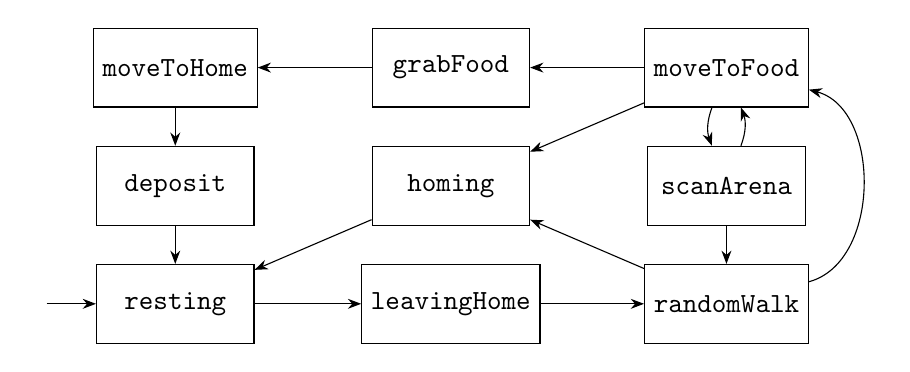
\begin{tikzpicture}[node distance=1.5cm and 3.5cm, on grid, auto]
\node[state] (deposit) {\texttt{deposit}};
\node[state, above=of deposit] (movetohome) {\texttt{moveToHome}};
\node[state, right=of movetohome] (grabfood) {\texttt{grabFood}};
\node[state, right=of grabfood] (movetofood) {\texttt{moveToFood}};
\node[state, right=of deposit] (homing) {\texttt{homing}};
\node[state, right=of homing] (scanarena) {\texttt{scanArena}};
\node[state, below=of deposit] (resting) {\texttt{resting}};
\node[left=5em of resting] (inv1) {};
\node[state, right=of resting] (leavinghome) {\texttt{leavingHome}};
\node[state, right=of leavinghome] (randomwalk) {\texttt{randomWalk}};

\path[->]
    (inv1) edge (resting)
    (resting) edge (leavinghome)
    (leavinghome) edge (randomwalk)
    (randomwalk) edge (homing)
    (homing) edge (resting)
    (randomwalk) edge[bend right=75](movetofood)
    (movetofood) edge (homing)
    (movetofood) edge[bend right=20] (scanarena)
    (scanarena) edge[bend right=20] (movetofood)
    (scanarena) edge (randomwalk)
    (movetofood) edge (grabfood)
    (grabfood) edge (movetohome)
    (movetohome) edge (deposit)
    (deposit) edge (resting);
\end{tikzpicture}
\caption{Abstract state transition system for the robot's foraging behaviour. The robot begins in a resting state, then searches for, collects, and deposits food.}
\label{fig:foraging-fsm}
\end{figure}
%
% \marienote{this caption could be a bit more descriptive: The robot begins in a resting state, then proceeds to walk around the arena, scanning, searching for, collecting and depositing food items...}
%
In the concrete transition system $\mathcal{M}$ the robot can remain in a given state for a configurable amount of time before it is forced to move to a next state. The transition system is specified concretely using \SMV{}, the language of the \nuXmv{} model checker~\cite{cavada2014}. We would like to prove that, after leaving the \texttt{resting} state, the robot will return to \texttt{resting} in at most 3 time units, represented by
%
\begin{equation}\label{eqn:max-return-to-resting-mtl}
\mathcal{M}\vDash\Box(\texttt{resting} \rightarrow \eventually{[1,3]}\texttt{resting})
\end{equation}
% \centereqn{\mathcal{M}\vDash\Box(\texttt{resting} \rightarrow \eventually{[1,3]}\texttt{resting})\label{eqn:max-return-to-resting-mtl}}
%
and translated from \MTL{} to \LTL{} as
%
\begin{equation}\label{eqn:max-return-to-resting-ltl}
\mathcal{M}\vDash\Box(\texttt{resting} \rightarrow X(\texttt{resting} \lor X(\texttt{resting} \lor X(\texttt{resting})))).
\end{equation}
% \centereqn{\mathcal{M}\vDash\Box(\texttt{resting} \rightarrow X(\texttt{resting} \lor X(\texttt{resting} \lor X(\texttt{resting})))).\label{eqn:max-return-to-resting-ltl}}
%
If this does not hold in the transition system, we would like to weaken the interval to produce a new, weaker property that does hold. Using \cegiw{}, we find in the first iteration that no suitable weakening of the interval exists based on the counterexample in \cref{fig:min-to-resting-cex}, which shows an infinite loop between the \texttt{scanArena} and \texttt{moveToFood} states. This suggests a mistake in the modelling of the system, as in the real world the robot's battery would run out of charge.
%
\begin{figure}[t]
\centering
% \begin{verbatim}
%                0 1 2 3 4 5
%   resting     │+│ │ │ │ │ │
%   leavingHome │ │+│ │ │ │ │
%   randomWalk  │ │ │+│ │ │ │
%   moveToFood  │ │ │ │+│ │+│
%   scanArena   │ │ │ │ │+│ │
%   =Lasso=              └─┘
% \end{verbatim}
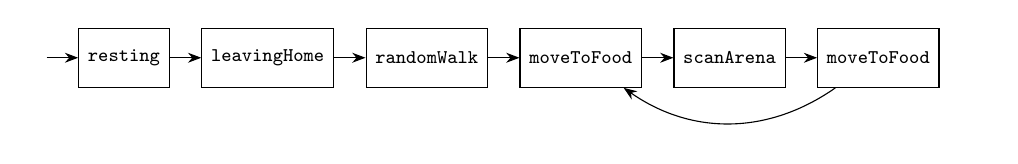
\begin{tikzpicture}[auto,node distance=4mm]
\node[cex] (1) {\scriptsize\texttt{resting}};
\node[left=of 1] (inv1) {};
\node[cex, right=of 1] (2) {\scriptsize\texttt{leavingHome}};
\node[cex, right=of 2] (3) {\scriptsize\texttt{randomWalk}};
\node[cex, right=of 3] (4) {\scriptsize\texttt{moveToFood}};
\node[cex, right=of 4] (5) {\scriptsize\texttt{scanArena}};
\node[cex, right=of 5] (6) {\scriptsize\texttt{moveToFood}};
\node[right=of 6] (inv2) {};

\path[->]
    (inv1) edge (1)
    (1) edge (2)
    (2) edge (3)
    (3) edge (4)
    (4) edge (5)
    (5) edge (6)
    (6) edge[bend right=325] (4);
\end{tikzpicture}
\caption{Infinite lasso counterexample trace for the property in \cref{eqn:max-return-to-resting-mtl}.}
\label{fig:min-to-resting-cex}
\end{figure}
%
We amend the design by including in the requirements the notion of a battery that decreases as transitions are taken. While we are in \texttt{randomWalk}, \texttt{scanArena}, or \texttt{moveToFood} --- in other words, searching for food --- we monitor the battery level, and if it decreases below a certain threshold we abort and return home to recharge. The modified state transition system is depicted in \cref{fig:foraging-fsm-modified}.
%
\begin{figure}[t]
\centering
\begin{tikzpicture}[node distance=1.5cm and 3.5cm, on grid, auto]
\draw[thick,dashed] ($(movetofood.north west)+(-0.3,0.3)$) rectangle ($(randomwalk.south east)+(0.3,-0.3)$) node [midway, above=2.25] {\texttt{battery monitor}};
\draw[->,thick,dashed] ($($($(movetofood.north west)+(-0.3,0)$)!0.5!($(randomwalk.south west)+(-0.3,0)$)$)$) -- (homing) node [midway, below] {\texttt{abort}};
\node[state] (deposit) {\texttt{deposit}};
\node[state, above=of deposit] (movetohome) {\texttt{moveToHome}};
\node[state, right=of movetohome] (grabfood) {\texttt{grabFood}};
\node[state, right=of grabfood] (movetofood) {\texttt{moveToFood}};
\node[state, right=of deposit] (homing) {\texttt{homing}};
\node[state, right=of homing] (scanarena) {\texttt{scanArena}};
\node[state, below=of deposit] (resting) {\texttt{resting}};
\node[left=5em of resting] (inv1) {};
\node[state, right=of resting] (leavinghome) {\texttt{leavingHome}};
\node[state, right=of leavinghome] (randomwalk) {\texttt{randomWalk}};

\path[->]
    (inv1) edge (resting)
    (resting) edge (leavinghome)
    (leavinghome) edge (randomwalk)
    (randomwalk) edge (homing)
    (homing) edge (resting)
    (randomwalk) edge[bend right=75](movetofood)
    (movetofood) edge (homing)
    (movetofood) edge[bend right=20] (scanarena)
    (scanarena) edge[bend right=20] (movetofood)
    (scanarena) edge (randomwalk)
    (movetofood) edge (grabfood)
    (grabfood) edge (movetohome)
    (movetohome) edge (deposit)
    (deposit) edge (resting);
\end{tikzpicture}
\caption{Abstract state transition system for the robot's modified foraging behaviour. The battery monitor is represented by the dashed section on the right.}
\label{fig:foraging-fsm-modified}
\end{figure}
%
\begin{figure}[t]
\centering
\begin{subfigure}[t]{0.5\textwidth}
    \centering
    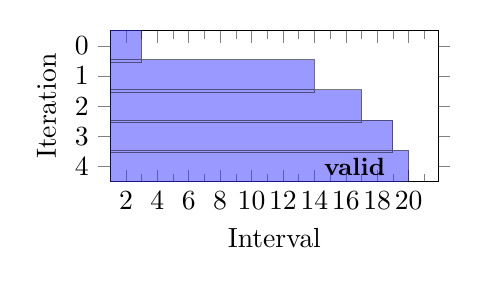
\begin{tikzpicture}
    \begin{axis}[
        xbar,
        xmin=1,
        width=5.75cm,
        height=3.5cm,
        xlabel={Interval},
        ylabel={Iteration},
        ytick=data,
        xtick distance=2,
        minor x tick num=1,
        x tick label as interval=false,
        y dir=reverse,
        ymin=-0.5,
        ymax=4.5,
        bar width=1.18em,
    ]
    \addplot+[black,fill=blue!80!white,opacity=0.5] coordinates {(20,4) (19,3) (17,2) (14,1) (3,0)};
    \node[
        anchor=west,
        font=\small,
    ] at (axis cs:14,4) {\textbf{valid}};
    \end{axis}
    \end{tikzpicture}
    \caption{Interval extension for \cref{eqn:max-return-to-resting-mtl}.}
    \label{fig:iterative-interval-extension}
\end{subfigure}%
\begin{subfigure}[t]{0.5\textwidth}
    \centering
    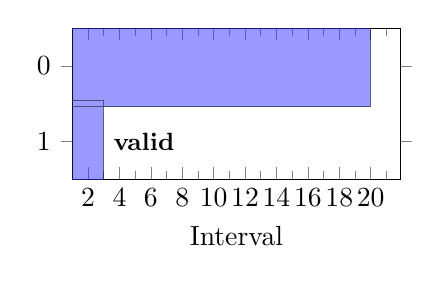
\begin{tikzpicture}
    \begin{axis}[
        xbar=1em,
        xmin=1,
        width=5.75cm,
        height=3.5cm,
        xlabel={Interval},
        ytick=data,
        xtick distance=2,
        minor x tick num=1,
        x tick label as interval=false,
        y dir=reverse,
        ymin=-0.5,
        ymax=1.5,
        bar width=2.95em,
    ]
    \addplot+[black,fill=blue!80!white,opacity=0.5] coordinates {(20,0) (3,1)};
    \node[
        anchor=west,
        font=\small,
    ] at (axis cs:3,1) {\textbf{valid}};
    \end{axis}
    \end{tikzpicture}
    \caption{Interval contraction for \cref{eqn:min-return-to-resting}.}
    \label{fig:iterative-interval-contraction}
\end{subfigure}
\caption{Iterative interval weakening to generate optimal, valid intervals.}
\end{figure}
%
We check our desired property (\cref{eqn:max-return-to-resting-mtl}) against our amended model, and can see in \cref{fig:iterative-interval-extension} that in four iterations of \cegiw{} we extended the interval, and ended with the optimal interval which was then verified to hold in the system. So, the optimal property that holds in our amended system is
\begin{equation}\label{eqn:max-return-to-resting-corrected}
    \mathcal{M}\vDash\Box(\texttt{resting} \rightarrow \eventually{[1,20]}\texttt{resting}).
\end{equation}
%
Another property we are interested in is not the maximum time that the robot can spend away from home, but the \emph{minimum}. We wish the robot to spend at least 20 time units away from home, formalised as
%
\begin{equation}\label{eqn:min-return-to-resting}
\mathcal{M}\vDash\Box((\texttt{resting}\land\eventually{[1,1]}\neg\texttt{resting}) \rightarrow \generally{[1,20]}\neg\texttt{resting}).
\end{equation}
%
Again, we check this against our modified model and can see in \cref{fig:iterative-interval-contraction} that it took only one iteration to contract the interval, reaching the optimal interval which was then verified to hold in the system as
%
\begin{equation}\label{eqn:min-return-to-resting-corrected}
\mathcal{M}\vDash\Box((\texttt{resting}\land\eventually{[1,1]}\neg\texttt{resting}) \rightarrow \generally{[1,3]}\neg\texttt{resting}).
\end{equation}
%
By using \cegiw{}, we first identified that the original specification had a design flaw that allowed unwanted infinite loops. After modifying the specification, we then deduced both the maximum time that the robot can stay away from home, as well as the minimum time.


\subsection{Applicability of Interval Weakening to Real-World Requirements (RQ2)}\label{subsec:case-studies}
%
\begin{table}[t]
\caption{Interval-weakenable requirements in \fret{} case studies.}
\label{table:weakenable-reqs-case-studies}
\centering
\begin{tabular}{ |l|r|r| } 
\hline
\textbf{Case study} & \textbf{Total requirements} & \textbf{Weakenable requirements} \\\hline
Mechanical lung ventilator~\cite{farrell2024} & 121 & 57 \\\hline
Autonomous drone~\cite{sheridan2025} & 62 & 19 \\\hline
Lift-plus-cruise aircraft~\cite{pressburger2023} & 49 & 29 \\\hline
Aircraft engine controller~\cite{farrell2022} & 42 & 0 \\\hline
Inspection rover~\cite{bourbouh2021} & 15 & 1 \\\hline
Grasping for debris removal~\cite{farrell2022a} & 20 & 0 \\\hline
Robotic patterns~\cite{vazquez2024} & 36 & 11 \\\hline
LMCP challenges~\cite{mavridou2020} & 74 & 7 \\\hline
\textbf{Total} & \textbf{419} & \textbf{124} \\\hline
\end{tabular}
\end{table}
%
\begin{figure*}[t]
    \centering
    \begin{subfigure}[t]{0.475\textwidth}
        \texttt{\textcolor{fret_condition}{upon ControlLoopStart}
        \textcolor{fret_component}{System}
        \textcolor{fret_shall}{shall}
        \textcolor{fret_timing}{within 12 milliseconds}
        \textcolor{fret_response}{satisfy ControlLoopFinish}}
        \caption{Autonomous drone requirement REQ018 describing the maximum time the control loop can take to complete.}
        \label{fig:example-fret-requirement-REQ018}
    \end{subfigure}%
    \hspace{1em}%
    \begin{subfigure}[t]{0.475\textwidth}
        \texttt{\textcolor{fret_condition}{if powerFailure}
        \textcolor{fret_component}{System}
        \textcolor{fret_shall}{shall}
        \textcolor{fret_timing}{for 120 minutes}
        \textcolor{fret_response}{satisfy !off}}
        \vspace{\baselineskip}
        \caption{Mechanical lung ventilator requirement FUN37 describing how long the system must stay on after power failure.}
        \label{fig:example-fret-requirement-FUN37}
    \end{subfigure}%
    \caption{Example \fretish{} requirements from the case studies. Both are taken from systems that are fully implemented and operational in real-world settings.}
\end{figure*}
%
In this section, we analyse existing requirements from a number of real-world case studies to assess how often interval weakening is applicable, and how weakened timing bounds can be interpreted in their respective domains. These requirements are formalised using the Formal Requirements Elicitation Tool (\fret{})~\cite{giannakopoulou2020a} and are written in \fretish{}, a structured natural language that can be translated to \MTL{}~\cite{giannakopoulou2021}. \fretish{} requirements can have a \texttt{\textcolor{fret_timing}{timing}} field, on which we can use interval weakening to weaken the requirement itself. The number of requirements that can be weakened using interval weakening per case study is shown in \cref{table:weakenable-reqs-case-studies}. As an example, the requirement in \cref{fig:example-fret-requirement-REQ018} from the autonomous drone case study~\cite{sheridan2025} uses the \texttt{\textcolor{fret_timing}{within 12 milliseconds}} timing which specifies that if the condition holds in one state, then the consequent must hold within the next twelve states (assuming that state transitions correspond to a millisecond of time passing). The \MTL{} translation of this timing corresponds to the \MTL{} temporal operator $\Diamond_{[0,12]}$, and so the requirement corresponds to
%
% We analyse the requirement sets from a number of case studies, which are formalised using the Formal Requirements Elicitation Tool (\fret{})~\cite{giannakopoulou2020a}. Requirements are written in \fretish{}, a structured natural language that can be translated to \MTL{}~\cite{giannakopoulou2021}. \fretish{} requirements can have a \texttt{\textcolor{fret_timing}{timing}} field, on which we can use interval weakening to weaken the requirement itself. The number of requirements that can be weakened using interval weakening per case study is shown in \cref{table:weakenable-reqs-case-studies}. As an example, the requirement in \cref{fig:example-fret-requirement-REQ018} from the autonomous drone case study~\cite{sheridan2025} uses the \texttt{\textcolor{fret_timing}{within 12 milliseconds}} timing which specifies that if the condition holds in one state, then the consequent must hold within the next twelve states (assuming that state transitions correspond to a millisecond of time passing). The \MTL{} translation of this timing corresponds to the \MTL{} temporal operator $\Diamond_{[0,12]}$, and so the requirement corresponds to
%
\begin{equation}\label{eqn:example-fret-requirement-REQ018}
\Box(\texttt{\textcolor{fret_condition}{ControlLoopStart}}\rightarrow \eventually{[0,12]}(\texttt{\textcolor{fret_response}{ControlLoopFinish}})).
\end{equation}
%
Under system degradation, for example if the onboard communications network is degraded so that commands take longer to reach control surfaces, we may not be able to guarantee this and so would have to weaken the property by extending the interval, giving more time for the system to run its control loop, with an example weakening in
%
\begin{equation}\label{eqn:example-fret-requirement-REQ018-weakened}
\Box(\texttt{\textcolor{fret_condition}{ControlLoopStart}}\rightarrow \eventually{[0,24]}(\texttt{\textcolor{fret_response}{ControlLoopFinish}})).
\end{equation}
%
An example requirement from the mechanical lung ventilator case study~\cite{farrell2024} is shown in \cref{fig:example-fret-requirement-FUN37}, and as the \fretish{} timing \texttt{\textcolor{fret_timing}{for 120 minutes}} corresponds to the \MTL{} temporal operator $\Box_{[1,120]}$, the corresponding \MTL{} property is
%
\begin{equation}\label{eqn:example-fret-requirement-FUN37}
\Box(\texttt{\textcolor{fret_condition}{powerFailure}} \rightarrow  \generally{[1,120]}(\neg\texttt{\textcolor{fret_response}{off}})).
\end{equation}
%
This is a regulatory requirement~\cite{iso2023} and so, if it does not hold in the degraded system, it is critical to know by exactly how much it is violated. We may only be able to guarantee that the ventilator will stay on for at most 90 minutes after \texttt{\textcolor{fret_condition}{powerFailure}}, producing the weakening
%
\begin{equation}\label{eqn:example-fret-requirement-FUN37-weakened}
\Box(\texttt{\textcolor{fret_condition}{powerFailure}} \rightarrow  \generally{[1,90]}(\neg\texttt{\textcolor{fret_response}{off}})).
\end{equation}
%
Of the 127 interval-weakenable requirements in \cref{table:weakenable-reqs-case-studies}, 116 can be weakened by interval extension as in \cref{eqn:example-fret-requirement-REQ018-weakened}, and 11 by interval contraction as in \cref{eqn:example-fret-requirement-FUN37-weakened}.

Several case studies in \cref{table:weakenable-reqs-case-studies} have few or no requirements that can be weakened with interval weakening. These requirements are typically liveness properties specified with the \texttt{\textcolor{fret_timing}{eventually}} timing, which cannot be weakened further, or safety properties specified with the \texttt{\textcolor{fret_timing}{always}} timing, for which interval weakening would not be appropriate. For example, from the grasping for debris removal case study~\cite{farrell2022a},
%
\begin{equation}\label{eqn:example-fret-requirement-always}
\texttt{\textcolor{fret_component}{SV}
\textcolor{fret_shall}{shall}
\textcolor{fret_timing}{always}
\textcolor{fret_response}{satisfy !collide(SV, TGT)}}.
\end{equation}
%
To answer \textbf{RQ2}, we have shown that interval weakening is applicable to a substantial proportion of existing temporal requirements, and that such weakenings have meaningful interpretations in safety-critical domains. We have also answered \textbf{RQ1} by using \cegiw{} to identify problems in a specification, and then deduce useful timing properties in the fixed system.



\section{Conclusion}\label{sec:conclusion}

We present \cegiw{}, a novel algorithm for weakening intervals in \MTL{} properties of degraded systems, and prove its correctness and optimality. We demonstrate how \cegiw{} can be used during the design phase to understand system limitations under degradation, and explore how the formalised requirements of a number of real-world systems may be weakened against real implementations. This shows the applicability of \cegiw{} in the design of safety-critical systems for understanding the impacts of system degradation.


% \marienote{say something about what the research querstion answers show}

\textbf{Future work.}
A current limitation is that we only weaken on the right-hand-side of intervals, when both left- and right-bound modifications can produce valid weakenings. Restricting to only right-bound modifications creates a total order over the search space, so there is always a single optimum when multiple choices exist. Expanding to both left- and right-bound modifications creates a partial order over generated intervals, and so choosing between intervals is much less obvious.

% Future work will also explore other types of weakening, making syntactic changes beyond intervals.



\printbibliography
% \clearpage
% \appendix

\section{Remaining Algorithm and Proofs}\label{sec:appendix}

\begin{algorithm}[t]
\SetAlgoNlRelativeSize{-1}
\caption{Directly weakening interval of $\mathcal{R}$}
\label{alg:weaken-direct-release}
\Function{\weakenreleasedirect($\psi_l$, $\psi_r$, $[a,b]$, $t$)}{
    $\bfin \gets \min(b, \rightidx_\pi(a))$ \\
    \For{$i \gets a$ \KwTo $\bfin$}{
        \If{$\pi,t+i\nvDash\psi_r$}{
            \If{$i=a$}{
                \Return $None$
            }
            \Return $[a,i-1]$
        }
        \If{$\pi,t+i\vDash\psi_l$}{
            \Return $[a,b]$
        }
    }
    \Return $[a,b]$
}
\end{algorithm}

Proof of \cref{lemma:weakening-algorithm-direct-release}, directly weakening the interval of $\mathcal{R}$.

\begin{proof}
    We take an arbitrary $t$. Our proof for \cref{alg:weaken-direct-release} uses the loop invariant that for all $j\in\covering_\pi(I)$ with $j<i$, we have that $\sat{\pi}{t+j}\psi_r$ and $\nsat{\pi}{t+j}\psi_l$. On first entry to the loop there is no such $j$, so this is trivially true. On reaching the end of the loop body, we know that $\nsat{\pi}{t+i}\psi_r$ and $\sat{\pi}{t+i}\psi_l$, and so in combination with the loop invariant we know that for all $j\in\covering_\pi(I)$ with $j\leq i$, we have that $\nsat{\pi}{t+j}\psi_r$ and $\sat{\pi}{t+j}\psi_l$. Thus the loop invariant is preserved. Suppose at the start of iteration $i$ the loop invariant holds. If $\nsat{\pi}{t+i}\psi_r$ then we have two cases:
    \begin{enumerate}
        \item If $i=a$ we have that $\nsat{\pi}{t+a}\psi_r$, so for all possible right-contractions $I'$ of $I$ we have that $\nsat{\pi}{t}\psi_l\release{I'}\psi_r$. Thus, there is no suitable interval and we return $None$.
    
        \item Otherwise, we return $I'=[a,i-1]$, which is an optimal right contraction of $I$. By the loop invariant we know for all $j\in\covering_\pi(I)$ with $j<i$ that $\sat{\pi}{t+j}\psi_r$, so we can conclude that $\sat{\pi}{t}\psi_l\release{I'}\psi_r$.
    \end{enumerate}
    If during this iteration $i$ we have that $\sat{\pi}{t+i}\psi_l$, then as this is after the above case is checked for we know that $\sat{\pi}{t+i}\psi_r$, and in combination with the loop invariant we have that $\sat{\pi}{t}\psi_l\release{I}\psi_r$. If we run the loop to completion, then by the loop invariant we know that for all $i\in\covering_\pi(I)$ we have $\sat{\pi}{t+j}\psi_r$. If $\covering_\pi(I)=I$ then we have
    $$
    \sat{\pi}{t}\psi_l\release{I}\psi_r
    $$
    If $\covering_\pi(I)=[a,\rightidx_\pi(a)]$ for some $a\in\N$, then by \cref{lemma:lasso-trace-coverage} we have that for all $i\in\N$ with $i\geq a$ we have $\sat{\pi}{t+j}\psi_r$, and so the above holds here too.
    %
    \qed
\end{proof}

\begin{algorithm}[t]
\label{alg:aux-until-right}
\SetAlgoNlRelativeSize{-1}
\caption{Weakening within $\mathcal{U}$ on the right}
\Function{\weakenuntilright($C$, $\phi$, $[a,b]$, $t$)}{
    $\bfin \gets \min(b, \rightidx_\pi(a))$ \\
    $intervals \gets [\;]$ \\
    \For{$i \gets a$ \KwTo $\bfin$}{
        $I \gets \weakenaux(C, t + i)$\\
        \If{$I \neq None$}{
            append $I$ to $intervals$
        }
        \If{$\pi, t + i \nvDash \phi$}{
            \textbf{break}
        }
    }
    \If{intervals is empty}{
        \Return $None$
    }
    \Return interval in $intervals$ with minimal absolute difference to $\Iorig$
}
\end{algorithm}

Proof of \cref{lemma:weakening-algorithm-inductive-until-right}, weakening within $\mathcal{U}$ on the right.

\begin{proof}
    We assume the inductive hypothesis $P(C)$, and want to prove $P(\phi\until{J}C)$. We take an arbitrary $t$. We distinguish two cases, according to whether $\triangle$ is $\mathcal{U}$ or $\mathcal{R}$. In either case, by the induction hypothesis each recursive call evaluates to either $None$ or an interval $I'$ related to $I$ by the corresponding relation (right-extension or \mbox{-contraction} respectively) such that $\sat{\pi}{t+t'} C[\psi\bintemporal{I'}\psi']$.
    
    We use the loop invariant that for all $j\in\covering_\pi(J)$ with $j<i$, we have that $\sat{\pi}{t+j}\phi$. On first entry to the loop there is no such $j$, so this is trivially true. On reaching the end of the loop body, we know for all $j\in\covering_\pi(J)$ with $j\leq i$ that $\sat{\pi}{t+j}\phi$, and so the loop invariant is preserved. Suppose at the start of iteration $i$ the loop invariant holds. If $\nsat{\pi}{t+i}\phi$ we exit the loop, and if the list of intervals is empty then by the loop invariant we know that there are no appropriate intervals $I'$ for any $j\in\covering_\pi(J)$ with $j<i$ for which $\sat{\pi}{t+j} C[\psi\bintemporal{I'}\psi']$, and so the same holds for $\sat{\pi}{t} (\phi\until{J}C)[\psi\bintemporal{I'}\psi']$.
    
    Otherwise, by the loop invariant we know that for all $j\in \covering_\pi(J)$ with $j<i$ we have $\sat{\pi}{t+j}\phi$ and, as we have passed the check above, that for at least one of these $j$ we have an interval $I'$ such that $\sat{\pi}{t+j} C[\psi\bintemporal{I'}\psi']$. Thus, we have
    $$
    \sat{\pi}{t} (\phi\until{J}C)[\psi\bintemporal{I'}\psi']
    $$
    %
    \qed
\end{proof}

\begin{algorithm}[t]
\label{alg:aux-release-right}
\SetAlgoNlRelativeSize{-1}
\caption{Weakening within $\mathcal{U}$ on the right}
\Function{\weakenreleaseright($C$, $\phi$, $[a,b]$, $t$)}{
    $\bfin \gets \min(b, \rightidx_\pi(a))$ \\
    $intervals \gets [\;]$ \\
    \For{$i \gets a$ \KwTo $\bfin$}{
        $I \gets \weakenaux(C, t + i)$\\
        \If{I $=$ None}{
            \Return $None$
        }
        append $I$ to $intervals$\\
        \If{$\pi, t + i \vDash \phi$}{
            \textbf{break}
        }
    }
    \Return interval in $intervals$ with maximal absolute difference to $\Iorig$
}
\end{algorithm}

Proof of \cref{lemma:weakening-algorithm-inductive-release-right}, weakening within $\mathcal{R}$ on the right.

\begin{proof}
    We assume the inductive hypothesis $P(C)$, and want to prove $P(C\release{J}\phi)$. We take an arbitrary $t$. We distinguish two cases, according to whether $\triangle$ is $\mathcal{U}$ or $\mathcal{R}$. In either case, by the induction hypothesis each recursive call evaluates to either $None$ or an interval $I'$ related to $I$ by the corresponding relation (right-extension or \mbox{-contraction} respectively) such that $\sat{\pi}{t+t'} C[\psi\bintemporal{I'}\psi']$.
    
    We use the loop invariant that for all $j\in\covering_\pi(J)$ with $j<i$, we have that $\sat{\pi}{t+j}\phi$. On first entry to the loop there is no such $j$, so this is trivially true. On reaching the end of the loop body, we know that for all $j\in\covering_\pi(J)$ with $j\leq i$ that $\sat{\pi}{t+j}\phi$, so the loop invariant holds. Suppose at the start of iteration $i$ the loop invariant holds. If $\nsat{\pi}{t+i}\phi$ we exit the loop, and if the list of intervals is empty then we know that there are no appropriate intervals $I'$ for any $j\in\covering_\pi(J)$ with $j<i$ for which $\sat{\pi}{t+j} C[\psi\bintemporal{I'}\psi']$, and so the same holds for $\sat{\pi}{t} (C\release{J}\phi)[\psi\bintemporal{I'}\psi']$.
    
    Otherwise, by the loop invariant we know that for all $j\in\covering_\pi(J)$ with $j<i$ we have $\sat{\pi}{t+j}\phi$, and, as we have passed the check above, that for at least one of these $j$ we have an interval $I'$ such that $\sat{\pi}{t+j} C[\psi\bintemporal{I'}\psi']$. Thus, we have
    $$
    \sat{\pi}{t}(C\release{J}\phi)[\psi\bintemporal{I'}\psi']
    $$
    %
    \qed
\end{proof}

\begin{algorithm}[t]
\label{alg:aux-release-left}
\SetAlgoNlRelativeSize{-1}
\caption{Weakening within $\mathcal{R}$ on the left}
\Function{\weakenreleaseleft($C$, $\phi$, $[a,b]$, $t$)}{
    $\bfin \gets \min(b, \rightidx_\pi(a))$ \\
    $intervals \gets [\;]$ \\
    \For{$i \gets a$ \KwTo $\bfin$}{
        \If{$\pi, t + i \nvDash \phi$}{
            \textbf{break}
        }
        $I \gets \weakenaux(C, t + i)$\\
        \If{$I \neq None$}{
            append $I$ to $intervals$
        }
    }
    \If{intervals is empty}{
        \Return $None$
    }
    \Return interval in $intervals$ with minimal absolute difference to $\Iorig$
}
\end{algorithm}

Proof of \cref{lemma:weakening-algorithm-inductive-release-right}, weakening within $\mathcal{R}$ on the right.

\begin{proof}
    We assume the inductive hypothesis $P(C)$, and want to prove $P(\phi\release{J}C)$. We take an arbitrary $t$. We distinguish two cases, according to whether $\triangle$ is $\mathcal{U}$ or $\mathcal{R}$. In either case, by the induction hypothesis each recursive call evaluates to either $None$ or an interval $I'$ related to $I$ by the corresponding relation (right-extension or \mbox{-contraction} respectively) such that $\sat{\pi}{t+t'} C[\psi\bintemporal{I'}\psi']$.
    
    We use the loop invariant that for all $j\in\covering_\pi(J)$ with $j<i$, we have that $\nsat{\pi}{t+j}\phi$ and that $I'=\weakenaux(C,\psi\bintemporal{I}\psi',t+j)$ is an interval such that $\sat{\pi}{t+j} C[\psi\bintemporal{I'}\psi']$. On first entry to the loop there is no such $j$, so this is trivially true. On reaching the end of the loop body, we know that $\weakenaux(C,\psi\bintemporal{I}\psi',t+i)\neq None$, and so by the induction hypothesis the recursive call must have produced a suitable interval $I'$. As we also know that $\nsat{\pi}{t+i}\phi$, the loop invariant is thus preserved for $j\in\covering_\pi(J)$ with $j\leq i$. Suppose at the start of iteration $i$ the loop invariant holds. If $I'=\weakenaux(C,\psi\bintemporal{I}\psi',t+i) = None$ then by the induction hypothesis we know that there is no suitable interval $I''$ for which $\sat{\pi}{t+i} C[\psi\bintemporal{I''}\psi']$, and by the loop invariant that there is no $j\in\covering_\pi(J)$ with $j<i$ for which $\sat{\pi}{t+j}\phi$. Thus, there is no interval $I''$ for which $\sat{\pi}{t} (C\until{J}\phi)[\psi\bintemporal{I''}\psi']$.
    
    If $\sat{\pi}{t+i}\phi$, then we exit the loop. As this check occurred after the recursive call to $\weakenaux$, we know that we have found at least one suitable interval. By the loop invariant we know that for all $j\in\covering_\pi(J)$ with $j<i$ we have an interval $I'$ such that $\sat{\pi}{t+j} C[\psi\bintemporal{I'}\psi']$. Applying \cref{lemma:extension-weakening-order} if $\triangle=\mathcal{U}$, or \cref{lemma:contraction-weakening-order} if $\triangle=\mathcal{R}$, we obtain a maximum interval $I''$ such that for all $j\in\covering_\pi(J)$ with $j\leq i$ we have $\sat{\pi}{t+j} C[\psi\bintemporal{I''}\psi']$, and so
    $$
    \sat{\pi}{t} (\phi\release{J}C)[\psi\bintemporal{I''}\psi']
    $$
    If we run the loop to completion, then by the loop invariant for each $i\in\covering_\pi(J)$ we have a suitable interval $I'$ where $\sat{\pi}{t+j} C[\psi\bintemporal{I'}\psi']$. If $\covering_\pi(J)=J$ then by the same reasoning as above we have a suitable maximum interval. If $\covering_\pi(J)=[a,\rightidx_\pi(a)]$ for some $a$ then by \cref{lemma:lasso-trace-coverage} this property holds for all $i\in\N$ with $i\geq a$, and so in this case we also have a maximum interval.
    %
    \qed
\end{proof}



\end{document}
